\documentclass[12pt,PhD]{muthesis}
\bibliographystyle{styles/vancouver}
\usepackage{cite}
\usepackage{graphics}
\usepackage{amstext}
\usepackage{amsmath}
\usepackage{algorithm}
\usepackage{algorithmic}
\usepackage{booktabs}
\usepackage{url} % typeset URL's reasonably
\usepackage{listings}

\newcommand{\unit}[2]{\ensuremath{#1\,\text{#2}}}
\newcommand{\cms}[1]{\ensuremath{#1\,\text{cms}^{\text{-1}}}}

\newcommand{\ms}[1]{\unit{#1}{ms}}
\newcommand{\msrange}[2]{\ensuremath{#1\text{--}#2\,\text{ms}}}
\newcommand{\mm}[1]{\unit{#1}{mm}}
\newcommand{\mv}[1]{\unit{#1}{mV}}
\newcommand{\degr}[1]{\ensuremath{#1^{\circ}}}

\newcommand{\supers}[1]{\ensuremath{^{#1}}}
\newcommand{\subs}[1]{\ensuremath{_{#1}}}
\newcommand{\ii}[1]{\ensuremath{\text{\emph{I}}_{\text{#1}}}}
\newcommand{\iip}[1]{\ensuremath{\text{\emph{I}}'_{\text{#1}}}}
\newcommand{\g}[1]{\ensuremath{\text{\emph{g}}_{\text{#1}}}}

\newcommand{\apd}[1][90]{APD\subs{#1}}
\newcommand{\apdr}[1][90]{APD\emph{r}{\scriptsize,#1}}


\newcommand{\nothree}{\ensuremath{\text{NO}_{3^{\text{-}}}}}

% picture predefines
\setlength{\unitlength}{1mm}

\newsavebox{\resistor}
\savebox{\resistor}(10,2)[bl]{
\put(0, 1){\line(1, 0){1}}
\put(1, 0){\line(0, 1){2}}
\put(1, 0){\line(1, 0){8}}
\put(1, 2){\line(1, 0){8}}
\put(9, 0){\line(0, 1){2}}
\put(9, 1){\line(1, 0){1}}
}

\newsavebox{\vresistor}
\savebox{\vresistor}(2, 10)[bl]{
\put(1, 0){\line(0, 1){1}}
\put(0, 1){\line(1, 0){2}}
\put(0, 1){\line(0, 1){8}}
\put(2, 1){\line(0, 1){8}}
\put(0, 9){\line(1, 0){2}}
\put(1, 9){\line(0, 1){1}}
}

\newsavebox{\cell}
\savebox{\cell}(10,10)[bl]{
\put(0, 0){\line(0, 1){10}}
\put(10, 0){\line(0, 1){10}}
\put(0, 0){\line(1, 0){10}}
\put(0, 10){\line(1, 0){10}}
}

% algorithmic package
\renewcommand{\algorithmiccomment}[1]{// #1}

\begin{document}

    \title{Developing Realistic Models of the Atrium and the P-Wave ECG}
    \author{Jonathan D. Stott}
    \principaladviser{Henggui Zhang}
    \school{School of Physics and Astronomy}

    \beforeabstract
    \prefacesection{Abstract}
%The University of Manchester\\
Jonathan David Stott\\
Doctor of Philosophy\\
Developing Realistic Models of the Human Atrium and the P-Wave ECG\\
23rd September 2009\\

Cardiac disease, including atrial fibrillation (AF), is one of the biggest causes of
morbidity and mortality in the UK, accounting for one third of all
deaths.\cite{foo}
Cardiac modelling is now a well established field.
Mathematical models offer a valuable way of gaining insight into the dynamic
behaviours of the heart, in normal and pathological conditions.
Great efforts have been put into modelling the ventricles, whilst the atria have
received less focus.
This thesis therefore concentrates on developing models of the atria.

In the first part of the thesis, I developed a simulation toolkit for
modelling myocyte electrophysiology and excitation waves in 1D \& 2D
tissues.
It includes optimisations such as adaptive stimulus protocols.
As examples of application, it is used to investigate effects of a novel anion
bearing current on atrial excitation and the effect of AF remodelling on atrial
myocyte electrical heterogeneity.

In the second part, a computationally efficient and anatomically based model of
the atria is constructed.
The 3D model includes heterogeneous, biophysically detailed
electrophysiology and conduction anisotropy.
The full model activates in \ms{121}\ in sinus rhythm, in
close agreement with clinical data.
The model is used, with the toolkit, to investigate the function effects of S140G
mutation in KCNQ1 which is associated with familial AF.

In the last half of the thesis, the 3D model forms the core of a boundary
element model of the P-wave Body Surface Potential (BSP).
The BSP model incorporates representions of the lungs and the heart blood masses.
Generated ECGs show qualitative agreement with clinical data.
Their morphology is as expected for a healthy person, with a lead II duration of
\ms{103}.
The BSP model is used to verify an existing algorithm for focal atrial
tachycardia location and in providing explanation for a novel clinical
phenomena, inverted P-waves at night.


Models of the human atria and body surface potential are constructed.
The models are validated against both experimental and clinical data.
These models are suitable to use as the platform for further research.



    Stuff happened
    \afterabstract
    \prefacesection{Acknowledgements}
    I would like to thank...
    \afterpreface
    

   \chapter{Introduction}

Cardiac disease is one of the biggest causes of death in the UK, causing over
one third of all deaths.
In addition to the deaths, many more people suffer the after effects of a heart
attack or live with the difficulties caused by heart failure~\cite{bhf2008}.
These figures are duplicated across much of the developed world.


\section{Motivations}

The atria have generally been neglected in studies, compared to the ventricles
at least.
Many more studies focus on ventricular tissue than atrial tissue, and many of
the atrial studies focus more on the pacemaker of the heart, than the atria as a
whole.
The atria have a complex electrophysiology and topology.
Whilst atrial dysfunction is rarely fatal, atrial arrhythmias are amongst the
most common cardiac diseases, reducing the quality of life for hundreds of
thousands of people.
They have recently been the focus of a variety of clinical and physiological
interest, interest which has not yet been reflected in cardiac modelling.

Mathematical modelling of the heart offers a way of gaining insight into the
cardiac processes and the mechanisms of cardiac disease.
It is a well established field of research with numerous international journals
and conferences discussing the findings.
Mathematical models allow physiological effects to be dissected and quantified
in ways that can be difficult for in vivo and in vitro experiments.
This can be used to inform both further experiments and clinical diagnosis and
treatment.

Despite these benefits, mathematical modelling has a number of downsides.
One of these is the technical expertise needed to model the heart.
It is a non-trivial programming task to setup a computer to solve the equations
of a mathematical model.
There are existing toolkits which solve this issue, but they have limitations.
Once the model has been set up, it needs to be used in a variety of experimental
protocols, to quantify the behaviour of the model and any abnormal conditions
the experimenter is interested in.
This task is both complicated, as the experimental protocols can involve complex
pacing patterns and require detailed measurements to be taken.
The task is also quite simple and repetitive, in that the same protocols are
wanted to assess many different cell types and abnormal conditions.
Finally, such protocols can vary between experimenters, making it harder to
compare results between different studies.

A second problem is that of clinical relevance.
Many computational experiments focus on simplified models of cardiac tissue in
one or two dimensions.
Whilst such experiments are useful for elucidating complex interactions, they
can be of limited use to a clinician.
The clinical electrocardiologist typically works with external tools such as the
ECG.
Clinical procedures are more expensive, stressful and sometimes dangerous.
Diagnosis therefore depends on using the ECG to infer the activity within the
heart.
Being able to link the electrical activity within a model to the observed
surface ECG can help with this, allowing an atrial model to be used to test
hypotheses with direct clinical relevance.


\section{Aims}

To address these issues, the thesis has three broad aims.
To construct a toolkit suitable for modelling cardiac tissue and particularly
atrial cells, to construct a model of the human atrium and the surface ECG and to
use the toolkit and the model in studies of the human atrium.

The cardiac simulation toolkit aims to address several problems of cardiac
modelling.
As a toolkit, it simplifies the basic set up for numerical experiments by
providing mathematical models ready to solve.
In addition, it will provide a number of experimental protocols, reducing the
repetitive work required to perform numerical experiments on cardiac tissue and
making cross-study comparisons easier.
The toolkit will also take advantage of optimisation techniques, making such
studies faster to undertake.

The model of the human atrium should allow for the modelling of some of the
complexities of atrial tissue; this includes regions of heterogeneous
electrophysiology and anisotropic conduction.
Through use of appropriately biophysically detailed models as the basis, it will
be suitable for use in studies such as electrophysiological remodelling or
inherited gene mutation.
Optimisation techniques will be used to make the problem computational
tractable.
The atrial model will be coupled to a representation of the human torso and used
as the basis of a forward calculation of the surface P-wave ECG.
This will allow studies of direct clinical relevance.


The tools and models will then be used in studies of atrial electrophysiology.
These will involve modelling the atrium on a number of scales from the single
cell through to the P-wave ECG.
The studies will incorporate both normal electrophysiology and a variety of
abnormal electrophysiological conditions.

\section{Synopsis}

This thesis consists of seven chapters.
In these chapters, a general background of the subject is given, before more
specific details of the toolkit developed are given.
There is then a section of experimental work with single cell, 1D, 2D and 3D
models.
A model of the body surface potential is then developed before being used in
experimental studies of the P-wave ECG.
Finally, conclusions and future work are given.

\textbf{Chapter 1}: This chapter.
A introduction to the motivations and aims of the thesis and a summary of the
chapters contained within.

\textbf{Chapter 2}: The physiological and mathematical background needed to
understand this thesis.
A description of the heart, with emphasis on the atria, is given, from the micro to the macro scale.
The normal functioning of the heart is described, both on cellular and whole
organ levels.
Mathematical models of cardiac tissue on all scales are introduced.
This includes a brief history of model development and information on both the
benefits and limitations of modelling.

\textbf{Chapter 3}: The development and components of a cardiac simulation
toolkit.
A description of the technology and techniques which have gone into the
development of the cardiac simulation toolkit.
Details are given of the experimental protocols modelled by the toolkit.
The features offered by the toolkit are compared with the offerings of existing
toolkits.

\textbf{Chapter 4}: Experimental studies in the atrium.
The atrial model developed in the thesis is presented, along with validating
information.
Experimental studies are presented, using the toolkit and simplified
versions of the whole atrium model.
These studies include a familial gene mutation, atrial fibrillation induced
remodelling and a novel current found in the human atrium.

\textbf{Chapter 5}: The body surface potential or forward problem.
The mathematics of computing the body surface potential from the electrical
potentials in the heart are given along with implementation details of the
software used to solve them and the torso model used.
The effects of internal inhomogeneities in the torso on the generated ECG are
investigated.
The generated ECGs are compared with clinical data from both twelve lead and
body surface potential mapping.

\textbf{Chapter 6}: Applications of the forward problem.
The body surface potential model is used in two clinical studies.
The first uses the model to validate an existing algorithm for predicting the
origin of focal tachycardia based on clinical data.
The second uses the model to investigate the causes of a novel clinical
phenomena, inverted P-waves at night.

\textbf{Chapter 7}: Discussions and Conclusions
This includes a look to the future and the many avenues for future research
offered by the toolkit and models developed in the thesis.


   \chapter{Constructing a Cardiac Simulation Toolkit}

\section{Experimental Protocols}



\subsection{Action Potential Duration}

\section{New Methods}

   \chapter{Modelling the Whole Atrium}

\section{Atrial Geometry}
\label{atrium:sec:geometry}

The atrial geometry used in the simulation studies presented here was based on
the visible human project female dataset.  The visible human dataset was
created from a pair of cadavers, set into wax and sliced into \mm{1}\ and
\mm{0.33}\ for the male and female bodies, respectively.  The geometric model
used here was extracted from the female dataset and so has a resolution of
\mm{0.33}.  The extracted geometry is segmented into different tissue types,
with distinct classifications for left and right atrium, the pectinate muscles,
the crista terminalis, the Bachmann bundle and the sino-atrial node, as shown in
figure \ref{atrium:geometry}.  The geometry has been used in numerous previous
simulation studies.  It was discretised via a finite differences approach, which
allows the whole atrium to be embedded in a block of $298\times269\times235$
nodes.  This gives it a total size of approximately 19 million total nodes,
although only approximately 1.6 million of those nodes correspond to excitable
cells.  The geometry also has simple fibre orientation in the pectinate muscles,
crista terminalis and Bachmann bundle.  The fibres are considered to always run
parallel to the local axis of the tissue bundle, as determined by principle
component analysis~\cite{Seemann2006}.

\section{Simulation Methods}

\subsection{Atrial Model}

The electrical activity at each of the nodes was described by the equations of
the Courtemanche--Ramirez--Nattel (CRN) of the human atrial
myocyte~\cite{crn98}.  This model, as previously described, is a second
generation model. It has 21 state parameters, representing ionic gating activations
and inactivations and intracellular concentrations of ionic species.  In the
model, the total current, \ii{ion} is made up of the contributions of numerous
channels
\begin{equation}
\label{atrium:crn}
\ii{ion} = \ii{Na} + \ii{K1} + \ii{to} + \ii{Kur} + \ii{Ks} + \ii{Kr} +
\ii{Ca,L} + \ii{p,Ca} + \ii{NaK} + \ii{NaCa} + \ii{b,Na} + \ii{b,Ca}
\end{equation}
where \ii{Na}, \ii{K1}, \ii{to}, \ii{Kur}, \ii{Ks}, \ii{Kr}, \ii{Ca,L},
\ii{p,Ca}, \ii{b,Na} and \ii{b,Ca}\ represent ionic currents and \ii{NaK}\ and
\ii{NaCa}\ are ion exchangers.  As a second generation model, the CRN model also
has a detailed calcium handling system which can influence the action potential
via its influence on the intracellular calcium concentration.

In some atrial simulations it was desirable to incorporate details of
electrophysiological heterogeneity to represent the difference in electrical
behaviour between atrial myocytes and the other cellular types present in the
geometry, the pectinate muscles and crista terminalis.  The parameters used for
heterogeneity were based on measurements taken by Feng et al.~\cite{feng1998}
of the canine atrium.  These were converted to parameters for the CRN model by
Seemann et al.~\cite{Seemann2004} and have been used in several simulation
studies~\cite{Seemann2006,Stott2008}.  They are shown in
table~\ref{atrium:het_params}.

\subsection{Monodomain Equation}

To simulate the propagation of electrical activity over the finite difference
geometry previously described, the mono-domain equation is used to describe the
changes in $V$ in time, $t$, the trans-membrane voltage.
\begin{equation}
\label{atrium:monodomain}
\frac{\partial V}{\partial t} = \nabla\cdot D \nabla V - \frac{\ii{ion}}{C_{m}}
\end{equation}
where $D$ is a tensor representing the diffusivity of electrical potential, \ii{ion} is described by the
CRN model (\ref{atrium:crn}), $C_{m}$ is the membrane capacitance and all other
symbols have their usual meanings.  Equation (\ref{atrium:monodomain}) is
advanced in time via the forward euler method with a timestep of \ms{0.05}.  For
simulations with isotropic conductivity between nodes a 7-node approximation of
the differential operator is used.  When anisoptropy is present, a 27-node
approximation is used.


   \chapter{The Body Surface Potential}

Whilst modelling the heart itself can provide valuable insights into the effects
of diseases and inherited conditions, as Chapters 2 and 3 show, a clinical
doctor cannot look at the heart's activity directly without a surgical
procedure.
Instead they must rely on external tools such as the echocardiogram and the
electro-cardiogram (ECG).
To reproduce the ECG with mathematical models, it is necessary to solve what is known as
the ``forward problem''.


\section{The Forward Problem}

To solve the forward problem, Maxwell's equations must be solved to determine the
field in the torso which arises from currents flowing within the heart.
Due to the nature of the problem---the finite size of the torso and the
relatively low frequencies involved---simplifying assumptions can be made.
The effects of propagation and of capacitive and inductive currents may be
neglected~\cite{Barnard1966}.
The situation must solve therefore becomes a quasi-static volume conductor
problem, which involves only tissue conductances.
The current flow in the torso, $\mathbf{J}$, is given by Ohm's law
\begin{equation}
\label{bsp:ohm}
\mathbf{J} = \sigma\mathbf{E} + \mathbf{J}^{i}
\end{equation}
where $\mathbf{E}$ is the electric field, $\sigma$ is the tissue conductivity
and $\mathbf{J}^{i}$ is an impressed, or applied, current.
The applied current term is included to allow for the presence of active sources and
is non-zero only at the locations of active sources, i.e. the heart.
Since the total current in (\ref{bsp:ohm}) is solenoidal (the net flow into or
out of any closed region is zero),
\begin{equation}
\label{bsp:ohm2}
\nabla \cdot \mathbf{J} = 0 = \sigma \nabla \cdot \mathbf{E} + \nabla \cdot \mathbf{J}^{i}
%= 0 = \sigma \bigtriangledown \cdot \mathbf{E} +
%    \bigtriangledown \cdot \mathbf{J}^{i}
\end{equation}
must be true.
As we are solving the quasi-static problem, $\mathbf{E}$ can be
found simply from the gradient of the scalar potential, $\phi$, as
\begin{equation}
\label{bsp:maxwell}
\mathbf{E} = - \nabla\phi
\end{equation}

If (\ref{bsp:maxwell}) is substituted into (\ref{bsp:ohm2}) then we obtain
\begin{equation}
\label{bsp:poisson}
\nabla^{2}\phi = \frac{\nabla \cdot \mathbf{J}^{i}}{\sigma}
\end{equation}
which can be recognised as Poisson's equation.
In an infinite homogeneous conducting medium, a solution to Poisson's equation
for the field at any given point, $\phi$, is~\cite{Plonsey1963}
\begin{equation}
\label{bsp:infinite}
\phi = \frac{1}{4 \pi \sigma} \int \frac{- \nabla \cdot
\mathbf{J}^{i} }{r} dV
\end{equation}
where $r$ is the (scalar) distance from the point of integration to the point at
which the field is being evaluated.

To account for the influence of the finite dimensions of the torso we can use
either a FEM or a BEM (See Chapter XXXX for a discussion
of the history of the two methods).
The derivation for the BEM method is based on Green's Theorem~\cite{Barr1966},
which states that for a volume, $V$, bounded by a surface, $S$, that
\begin{equation}
\label{bsp:green}
\int_{V} \left(\phi \nabla^{2}\psi - \psi \nabla^{2}\phi  \right) dV =
\int_{S} \left( \phi \nabla \psi - \psi \nabla \phi \right) \cdot d\mathbf{S}
\end{equation}
where $\phi$ and $\psi$ are scalar functions of position.
If $\phi$ is the electrical potential and $\psi$ is set as $\frac{1}{r}$ where
$r$ is $|\mathbf{r'}-\mathbf{r}|$.
Here, $\mathbf{r'}$ is a vector to an arbitrary point in the volume $V$ at which
we wish to evaluate the field and $\mathbf{r}$ is a vector to an elemental
volume, $dv$, somewhere within the volume $V$.
Using (\ref{bsp:poisson}) we have
\begin{equation}
\label{bsp:greenandpoisson}
\int_{V}
    \left(
        \phi \nabla^{2}\left(\frac{1}{r}\right) -
        \frac{1}{r} \nabla^{2}\frac{\left(\nabla \cdot \mathbf{J}^{i} \right)}{\sigma}
    \right)
dV =
\int_{S}
    \left(
        \phi \nabla \left(\frac{1}{r}\right) -
        \left(\frac{1}{r}\right) \nabla \phi
    \right)
\cdot d\mathbf{S}
\end{equation}

The del operator in (\ref{bsp:poisson}) operates on the unprimed (source) coordinates.
Now,
\begin{equation}
\label{bsp:oneoverr}
\nabla^{2}\left(\frac{1}{r}\right) =
\nabla^{2}\left(\frac{1}{|\mathbf{r'}-\mathbf{r}|}\right) =
-4\pi\delta\left(\mathbf{r'}-\mathbf{r}\right)
\end{equation}
where $\delta$ represents the dirac delta function.  The surface $S$ is the body
surface and so on $S$ $\nabla\phi \cdot d\mathbf{S} = 0$ to a very good
approximation.  (\ref{bsp:poisson}) becomes, after substitution and
rearrangement,
\begin{equation}
\label{bsp:substituted}
\phi\left(\mathbf{r'}\right) =
\frac{1}{4 \pi \sigma}\int_{V} \frac{\nabla \cdot \mathbf{J}^{i}}{r}dv - 
\frac{1}{4 \pi}\int_{S} \phi\left(\mathbf{r}\right)
\nabla\left(\frac{1}{r}\right) \cdot \d\mathbf{S}
\end{equation}


   \chapter{Applications Of The Forward Problem}

The ECG is the first tool cardiac doctors turn to when diagnosis of a problem is
required.
ECG machines can be found in almost every hospital in the world.
A model of the atria and the surface potentials developed by the excitation of
the model can be used to guide diagnosis of a variety of conditions.
This can reduce the need for surgical procedures or suggest when they are
essential.

Whilst the inverse problem promises to reproduce the potentials on the heart
from the potentials on the surface, the technique has limitations.
For accurate solutions, patient specific geometries have to be constructed from
MRI scans.
There is also a need for complex lead systems, sometimes featuring more than two
hundred leads.
Also, many of the inverse techniques rely on `smooth' propagation patterns to
reduce the uncertainties in the technique which may not be found in pathological
cases.
A device which can perform such calculations automatically is a long way off,
both in terms of computational power required and complexities to resolve.

By contrast, diagnostic guides based on a forward solution can be of use to any
doctor.
They can also be used to further validate simulation studies of genetic or
diseased conditions, by comparison of the generated ECGs with those recorded
from real patients.
This chapter explores some of these predictions, using the model developed in
the previous chapter.

\section{Inverted P-Waves at Night}

Recently an observation was made~\cite{BoyettPrivate}\ concerning patients under
24 hour ECG monitoring.
It was noted that some patients exhibited inverted P-waves at night.
That is to say, if the patient showed a positive P-wave in leads II and aVF
during the day, then at night the P-wave would be negative in leads II and aVF.
These patients had no known heart disease or conduction defects.
This phenomena has not been reported in the literature.

There is evidence~\cite{Shibata2001,Boineau1988,Dobrzynski2005} that the pacemaker is not a
small and discrete area of the atrium, but is instead distributed along the
length of the crista terminalis.
The presence of certain drugs and hormones, most notably acetylcholine, can cause
the site of the leading pacemaker to move down the pace maker complex.
Acetylcholine is released by what is know as increased `vagal tone'.
This has been observed to happen at night.
It was hypothesised that a pacemaker shift induced by this increased vagal tone
might lead to the observed P-wave inversion.

\subsection{Methods}

In the absence of a model for the distributed pacemaker complex in the human
heart, the direct effects of acetylcholine could not be investigated.
Instead, using the model presented in the previous chapter, several sites were
located along the crista terminalis.
These sites had a radius of 15 nodes (or approximately \mm{5}--although this
varied depending on the thickness of the atrial wall at the pacing site), and
therefore were approximately the same size as the sino-atrial node.
These sites are shown in figure~\ref{fig:forward:ct_sites}.
Each of these sites was stimulated via the same protocol used to stimulate the
sinus node in the original model and then the electrical excitation waves were
allowed to propagate without interference.

ECGs were computed from the patterns of electrical excitation in the atrium.
These were compared to the sinus rhythm ECGs computed in the previous chapter.
In addition, using a so called `inverse Dower' method after Edenbrandt and
Pahlm~\cite{Edenbrandt1988}, the orthogonal components of the ECG were computed
and used to construct representations of the heart
vector~\cite{Frank1956,MacFarlane1989a} ECG (VECG).
To perform the inverse dower transformation, a matrix that has been optimized for
the P-wave (shown in Table~\ref{tbl:forward:idparams}) was
used~\cite{Guillem2007}.


\begin{table}
\caption[Inverse Dower Factors]{
\label{tbl:forward:idparams}
Factors to construct the Frank VECG from the standard 12 lead ECG set.
Parameters optimised to accurately reproduce the P-wave heart
vector~\cite{Guillem2007}.
Each of the 8 leads are multiplied by the given parameters to provide the
orthogonal Frank lead.
}
\begin{center}
\begin{tabular}{c c c c c c c c c}
\toprule
& $\text{V}_{\text{1}}$ &$\text{V}_{\text{2}}$ & $\text{V}_{\text{3}}$ &
$\text{V}_{\text{4}}$ & $\text{V}_{\text{5}}$ & $\text{V}_{\text{6}}$ & I & II \\
\midrule
X & $-0.266$ & $\:0.027$ &  $\:0.065$ & $\:0.131$ & $\:0.203$ & $\:0.220$ & $\:0.370$ & $-0.154$ \\
Y & $\:0.088$ &  $-0.088$ & $\:0.003$ & $\:0.042$ & $\:0.047$ & $\:0.067$ & $-0.131$ & $\:0.717$ \\
Z & $-0.319$ & $-0.198$ & $-0.167$ & $-0.099$ & $\:0.009$ & $\:0.060$ & $\:0.184$ & $\:0.114$ \\
\bottomrule
\end{tabular}
\end{center}
\end{table}

\subsection{Results}

\subsubsection{Activation Sequence}

The activation sequences of the atria after pacing from the sinus node, and the
three sites along the crista terminalis are shown in
figure~\ref{fig:forward:inverse:active}\ as isochronal colour maps.
Time goes from red, at \ms{0}, to blue, at \ms{150}.
The site of first activation obviously shifts depending on the stimulus
location.
In addition, as the stimulus site moves away from the sinus node, the time to
total activation of the atria increases.

\begin{figure}
\begin{center}
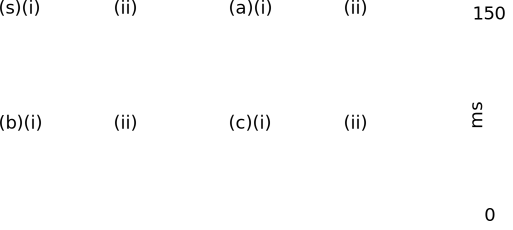
\includegraphics{figures/forward/inverted_p_wave/activation_sequence}
\end{center}
\caption[Activation sequences from pacing sites along the CT]{
\label{fig:forward:inverse:active}
Atrial activation sequences obtained from different pacing sites.
Shown are the activation sequences resulting from pacing at the sinus node, (s),
and the three crista terminalis sites A--C (a--c).
Activation times are represented by colours, going from red at $\leq$\ms{5}\
through green, \ms{75} to deep blue at \ms{150}.
Contours are every \ms{5}.

There are two views shown for each pacing site.
(i), a view of the right atrial surface with the superior vena cava at the top
of the right atrial surface and the tricuspid valve at the base.
In this view, the crista terminalis runs approximately vertically.
(ii), a view up into the atrial cavities through the valve openings.
The ribbed structures of the pectinate muscles are visible through the tricuspid
valve as they extend off the crista terminalis on the left of the panel.
The right and left atrial appendages are to the top of the panels.

In panel (s) the sinus rhythm activation sequence is visible with rapid
conduction along the crista terminalis and pectinate muscles.
The Bachmann's bundle meanwhile rapidly conducts the excitation to the left
atrium.
In both atria, the appendages are amongst the last regions to depolarise.

In panel (a), the activation sequence has shifted slightly down the crista
terminalis.
The pectinate muscles and crista terminalis still have a large influence on the
propagation.
In both atria, the appendages are the last regions to depolarise.

In panel (b), the activation sequence is shifted a long way down the crista
terminalis.
The Bachmann's bundle is no longer the site of first activation of the left
atrium.
Total time to activate is noticeably delayed.

In panel (c), the activation sequence is shifted a long way down the crista
terminalis.
Total time to activate is noticeably delayed in the left atrium.
The Bachmann's bundle is no longer the site of first activation, instead the
area close to the coronary sinus is first activated.
}
\end{figure}

The sinus node activation sequence,
figure~\ref{fig:forward:inverse:active}(s)(i, ii), starts high on the right
atrium, close to the superior vena cava.
Conduction is especially rapid down the crista terminalis and along the
pectinate muscles, visible as the more widely spaced isochrones along these
structures.
The Bachmann bundle, meanwhile, conducts the electrical excitation to the left
atrium, where it then starts to spread over the left atrial endocardial surface.
In the right atrium the activation finishes, after approximately \ms{80}\ have
elapsed since stimulation started, with the activation of the ring around the
tricuspid valve and the right atrial appendage.
In the left atrium, the far extremities of the left atrial appendage and the far
side of the mitral valve to the Bachmann bundle are activated at approximately
\ms{120}, completing the activation of the atria.

The activation sequence from site A,
figure~\ref{fig:forward:inverse:active}(a)(i, ii), starts high on the right
atrium in the region where the pectinate muscles are branching from the crista
terminalis.
This leads to rapid conduction down the pectinate muscles and in both directions
along the crista terminalis.
The Bachmann bundle conducts the excitation to the left atrium, where it starts
to spread.
The activation of the right atrium finishes with the activation of the right
atrial appendage and then region between the septum and the tricuspid valve.
Activation of the left atrium completes in \ms{132}\ after the initial stimulus
on the edge of the left atrial appendage and the mitral valve.

Pacing from site B leads to the activation sequence depicted in
figure~\ref{fig:forward:inverse:active}(b)(i, ii).
The activation sequence starts lower on the crista terminalis, and is conducted
in both directions along the muscle ridge.
The pectinate muscles also influence the conduction, although the excitation
wavefront reaches them later.
Excitation still reaches the left atrium through the Bachmann bundle, although
it is also conducted through the septum close to the inferior vena cava.
The last point to be excited in the right atrium is still the appendage.
In the left atrium, the last activation comes at \ms{140}.
The left atrial appendage and the sheaths of the pulmonary veins both finish
activating at this time.

The activation sequence which results from pacing from site C is shown in
figure~\ref{fig:forward:inverse:active}(c)(i, ii).
The activation sequence starts low on the right atrium and spreads in all
directions, but is faster travelling up the crista terminalis.
The pectinate muscles, when the excitation wave reaches them, also have a
noticeable effect, speeding activation of the right atrium.
Once again, the left atrium appears to be excited in two places, both by the
bachmann's bundle and close to the inferior vena cava through the septum.
The right atrial appendage is the last region of the right atrium to be excited.
In the left atrium, the extremities of the appendage and the pulmonary vein
sheaths are the last to be excited, as well as the region close to the mitral
valve.
This activation starts at approximately \ms{140}.

All of the activation sequences are approximately normal, in that they travel
from right to left.
The further the stimulus site is removed from the sinus node, the longer
excitation tends to take.


\subsubsection{Twelve Lead ECG}

The ECGs from the three pacing locations along the CT are shown in
figure~\ref{fig:forward:inverse:ecgs}\ with the sinus rhythm P-wave ECG for
comparison.
A summary of the lead deflections for the four cases and sinus rhythm are
presented in table~\ref{tbl:forward:inverse:ecgs}.
There is a clear evolution of the P-wave morphology visible as the pacing site
is moved down the crista terminalis.

\begin{table}
\caption[Lead classification under pacing from different locations]{
\label{tbl:forward:inverse:ecgs}
Lead classification after pacing from different locations.
Leads are classified based on the criteria used by
Kistler~et~al.~\cite{Kistler2006}.
A positive P-wave is denoted by a $+$ sign, a negative P-wave by a $-$ sign and
a biphasic one by $\sim$.
Site denotes the pacing site, where S is the sinus node and Sites A--C are as
indicated in Figure~\ref{fig:forward:ct_sites}.
}
\begin{center}
\begin{tabular}{c c c c c c c c c c c c c}
\toprule
Site & I & II & III & aVR & aVL & aVF & $\text{V}_{\text{1}}$ &$\text{V}_{\text{2}}$ & $\text{V}_{\text{3}}$ & $\text{V}_{\text{4}}$ & $\text{V}_{\text{5}}$ & $\text{V}_{\text{6}}$\\
\midrule
S   & $+$ & $+$ & $\sim$ & $-$ & $+$ & $+$ & $-$ & $+$ & $+$ & $+$ & $+$ & $+$ \\
A   & $+$ & $+$ & $\sim$ & $-$ & $+$ & $\sim$ & $-$ & $+$ & $+$ & $+$ & $+$ & $+$ \\
B   & $+$ & $\sim$ & $-$ & $-$ & $+$ & $-$ & $+$ & $+$ & $+$ & $+$ & $+$ & $+$ \\
C   & $+$ & $-$ & $-$ & $-$ & $+$ & $-$ & $+$ & $+$ & $+$ & $+$ & $+$ & $+$ \\
\bottomrule
\end{tabular}
\end{center}
\end{table}

\begin{figure}
\begin{center}
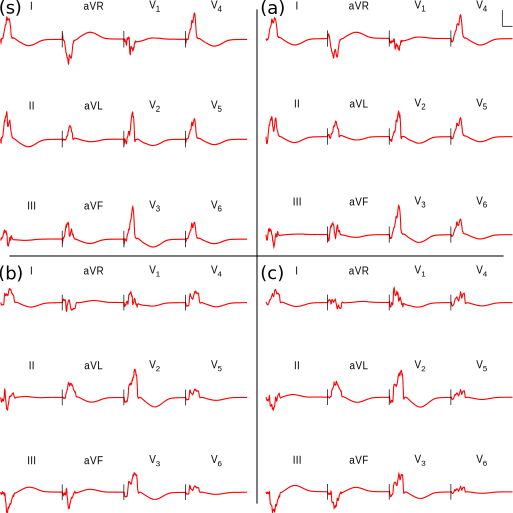
\includegraphics{figures/forward/inverted_p_wave/inverted_pwave_ecg}
\end{center}
\caption[12 Lead ECG traces from pacing sites along the CT]{
\label{fig:forward:inverse:ecgs}
Twelve lead ECG recordings obtained from the model after pacing at the sinus
node, (s) and the three pacing sites A--C (a--c).
Shown is one complete P-wave and $\text{T}_{\text{P}}$ wave, pacing at a rate of
\unit{60}{bpm}.
The scale is the same for all traces, indicated in the top right of panel (a).
The P-wave is positive in leads II and aVR after pacing from the sinus node.
It is positive in leads II and aVR after pacing from site A.
Pacing from site B leads to a negative P-wave in lead aVF and a biphasic P-wave
in lead II.
Site C shows negative P-waves in both leads II and aVR.
}
\end{figure}


The P-wave ECG for pacing from the sinus node,
figure~\ref{fig:forward:inverse:ecgs}(s), is positive in leads II and aVF.
Leads I, aVL and $\text{V}_{\text{2--6}}$ are also positive.
Leads aVR and $\text{V}_{\text{1}}$ are negative.
Lead III is biphasic.
The largest positive lead is $\text{V}_{\text{3}}$, which attains a potential
difference of \mv{+0.390} and the largest negative lead is aVR,
which attains a potential difference of \mv{-0.299}.
The definite positive P-waves in the last 5 precordial leads,
$\text{V}_{\text{2--6}}$, suggest normal propagation through the atrium, with
depolarisation travelling from right to left.
The cardiac axis is approximately $+30^\circ$ in the frontal plane.


Pacing from site A (figure~\ref{fig:forward:inverse:ecgs}(a)), the P-wave ECG is
positive in leads II and  aVF.
Leads I, aVL and $\text{V}_{\text{2--6}}$ are also positive.
Lead aVR and $\text{V}_{\text{1}}$ are negative.
Lead III is biphasic.
The largest positive lead is $\text{V}_{\text{3}}$, which attains a potential
difference of \mv{+0.358} and the largest negative lead is aVR,
which attains a potential difference of \mv{-0.240}.
The definite positive P-waves in the last 5 precordial leads,
$\text{V}_{\text{2--6}}$, suggest normal propagation through the atrium, with
depolarisation travelling from right to left.
The cardiac axis is approximately $+30^\circ$ in the frontal plane.
There is a very prominent notch visible in both leads II and aVF, caused by ...
foo!

Pacing from site B (figure~\ref{fig:forward:inverse:ecgs}(b)), the P-wave ECG is
biphasic in lead II and negative in lead aVF.
Leads I, aVL and $\text{V}_{\text{1--6}}$ are positive.
Lead III and aVR are negative.
The largest positive lead is $\text{V}_{\text{2}}$, which attains a potential
difference of \mv{+0.356} and the largest negative lead is III,
which attains a potential difference of \mv{-0.258}.
The definite positive P-waves in the last 5 precordial leads,
$\text{V}_{\text{2--6}}$, suggest normal propagation through the atrium, with
depolarisation travelling from right to left.
The propagation up the crista terminalis, not down it, is evidenced in the
positive P-wave in $\text{V}_{\text{1}}$.
The cardiac axis is approximately $-30^\circ$ in the frontal plane, due to
activation now travelling up the atrium, rather than down.


Pacing from site C (figure~\ref{fig:forward:inverse:ecgs}(c)), the P-wave ECG is
negative in lead II and lead aVF.
Leads I, aVL and $\text{V}_{\text{1--6}}$ are positive.
In addition to leads II and aVF, lead III and lead aVR are negative.
The largest positive lead is $\text{V}_{\text{2}}$, which attains a potential
difference of \mv{+0.343} and the largest negative lead is III,
which attains a potential difference of \mv{-0.263}.
The positive P-waves in leads $\text{V}_{\text{2--6}}$ suggest that the
propagation is still from right to left, although the low amplitudes in the
later leads suggests that this is not as uniform as in the previous cases.
The propagation up the crista terminalis, not down it, is evidenced in the
positive P-wave in $\text{V}_{\text{1}}$.
The cardiac axis is approximately $-60^\circ$ in the frontal plane, due to
activation now travelling up the atrium, rather than down.

As the pacing site moves down the crista terminalis there is an evolution of the
P-wave, which is visible in all leads.
As a result of the shift, the cardiac axis shifts through about $90^\circ$
anti-clockwise from the sinus direction of $+30^\circ$.
The P-wave duration increases slightly as the crista terminalis increases,
highlighting the importance of the specialized conduction structures of the
heart in rapidly conducting the excitation wave.


\subsubsection{Derived Vector ECGs}

The derived vector ECG plots are shown for the frontal plane in
figure~\ref{fig:forward:inverse:vec_front} and in the transverse plane in
figure~\ref{fig:forward:inverse:vec_trans}.
Again, the sinus rhythm is included in both figures for reference.
The colour of the vector loop represents the passage of time and is coloured
from purple, at \ms{0}, through blue, green, yellow and ending up red at
\ms{500} after initiation of the P-wave.

The vector loop in the frontal plane for sinus rhythm is shown in
figure~\ref{fig:forward:inverse:vec_front}(s).
The vector loop is inscribed in an anti-clockwise direction.
The efferent limb is at approximately \degr{+60}, before it loops up to its
maximal extension at approximately \degr{+45}.
There is a small sub-loop on the afferent limb as the vector trace reaches the
\degr{+30}\ line.
This is possibly caused as the excitation wavefront loops around the tricuspid
valve and the right atrial appendage depolarises.
The $\text{T}_{\text{P}}$ wave is visible as a small anti-clockwise loop,
aligned at approximately \degr{-135}.
The initial deflection along the same line is an artefact of the stimulus
protocol.

The frontal plane vector loop for pacing from site A,
figure~\ref{fig:forward:inverse:vec_front}(a), is inscribed in an anti-clockwise
direction in general.
The main axis of the loop is at approximately \degr{+35}.
The efferent limb is aligned at approximately \degr{+60}, along the line of lead
II.
The afferent limb shows a large loop, which corresponds to the notch in the 12
lead ECG.
The small shift in the pacing site appears to have a relatively large influence
on the 
The $\text{T}_{\text{P}}$ wave is visible as a small loop, aligned at
approximately \degr{-150}.

Pacing from site B produces the frontal plane vector loop in
figure~\ref{fig:forward:inverse:vec_front}(b).
The loop is a figure-of-eight which is initially anti-clockwise.
The main axis of the loop is at approximately \degr{+0}.
The efferent limb is initially aligned at \degr{+30}\ before it sweeps around to
\degr{-60}.
The afferent limb loops back on itself, to \degr{-10} before it returns to the
centre.
The $\text{T}_{\text{P}}$ wave is visible as a small anti-clockwise loop, aligned at
approximately \degr{+150}.
The loop is smaller than that which is observed in the two preceeding pacing
locations.

The frontal plane vector loop from pacing at site C is shown in
figure~\ref{fig:forward:inverse:vec_front}(c).
The loop is open, and inscribed in a clockwise direction.
The main axis of the loop is aligned at approximately \degr{-40}.
The efferent limb oscillates as it travels out along an approximately
\degr{-60}\ vector.
The loop then sweeps down to \degr{-30}, before the afferent limb oscillates as
it returns to 0.
The $\text{T}_{\text{P}}$ is a small clockwise loop at an angle of \degr{+150}.
The loop from site C is the smallest of the loops.

As the pacing site moves down the crista terminalis there are clear changes in
the morphology and principle axis of the P-wave frontal vector loop.
The axis shift which could be determined from the 12 lead ECG was clearly
highlighted.
The vector loops also show the reduction in amplitude of the P-wave as the
pacing location is moved down the crista terminalis, possibly caused by the
generally slower speed of activation.

\subsection{Discussion}

As the stimulus site moves down the crista terminalis the patterns of electrical
activation in the atrium change noticeably.
The focal point of excitation obviously moves down the crista terminalis to
follow this.
It is also interesting to note the similarities.
Despite the shifting activation site, the right atrial appendage and the region
between the tricuspid valve and the atrial septum are always the last to
activate in the right atrium.
In the left atrium, the appendage also activates last in all cases.

As the pacing site moves away from the sinus node, the total activation time
increases.
However, total activation times remain within those observed clinically by
Lemery~et~al.~\cite{Lemery2004}\ for all three pacing locations away from the
sinus node.
The activation patterns are similar to those observed by
Bouineau~et~al.~\cite{Bouineau1988}\ as the pacing location moves, although the
Bouineau data does not include single activations away from the sinus node.

The latter two sites (B \& C), which are low on the crista terminalis, appear to
reach the left atrium in part through a site which emerges close to the coronary
sinus~\cite{Platonov2007,Platonov2008,Markides2003,Lemery2004}.
There is no specialist inferior intra-atrial conduction pathway in the model
however.
Conduction along this lower route is therefore at the normal bulk tissue rate.
It is possible if this were treated specially in the model total activation
times would be reduced.

The ECGs generated from the model also show an evolution as the stimulus site
moves down the crista terminalis.
This change is more visible in the limb leads than in the precordial leads.
This is to be expected, as the propagation remained from right to left in all
cases, but whether it is travelling up or down the atria changes as the pacing
site does.
The P-waves in leads II and aVF is positive in during sinus rhythm, and both
gradually invert as the pacing site shifts down the crista terminalis, as
hypothesised.

As the pacing site moves away from the sinus node, the P-wave duration also
increases.
Especially for the lower crista terminalis sites (B \& C), the duration exceeds
normal P-wave limits~\cite{Lemery2004,Macfarlane1989}.
It is possible that a more detailed intra-atrial conduction system, including an
inferior pathway would reduce total conduction time, and therefore P-wave
duration in these cases.

The P-wave vector loops are similar to those observed in clinical
studies~\cite{Carlson2005,Holmqvist2007,Havmoller2007,Guillem2007}, although the typical
presentation of such loops as monochromatic does make comparison of the timing
information and direction of inscription hard.
They make it quite obvious that the cardiac axis shifts as the pacing location
does.
The morphology of the loops can be used to gain further clues, such as with the
initial rise and then fall visible in the Site B frontal vector loops.

The limitations of the body surface potential model have been discussed
previously (Section X.X.X).
Of particular importance to this study is the lack of a distributed sinus node
model~\cite{Yamamoto2007,Dobrzynski2005}\ for the human atrium.
However, pacemaker shift under the influence of
acetylcholine~\cite{Shibata2001}\ has been observed in rabbits and in
humans~\cite{Opthof1988}\ so it seems plausible as a mechanism for the shifts
and associated P-wave inversions.
The use of an inverse dower matrix to obtain the frank leads rather than
directly measuring them was chosen to allow more direct comparison with clinical
data, which is often only for the standard twelve leads.
The selection of the correct transform matrix is
important~\cite{Guillem2007,Luo1991,Hyttinen1995}\ and it is possible that the
vector loop accuracy could be improved by the use of a transformation matrix
optimised for the body surface potential model.
Alternatively a true frank lead system, or a hybrid model could be constructed.

\subsection{Conclusions of the Inverted P-Wave Study}

The hypothesis that P-wave inversion could be caused by pacemaker shift in the
human sinus node seems to be plausible.
Progressive shift of the pacemaker site down the sinus node leads to progressive
inversion of the observed P-waves in leads II and aVF.
In addition, this shift is accompanied by other changes which do not stray too
far from normality.
This is important, as the shift was originally observed in those with no
diagnosed cardiac disorders.
Further investigation is merited, once an appropriate model of the distributed
sino-atrial node complex can be integrated into the atrial model.

This study shows that the body surface potential model can be used for a study
which involves conditions that begin to deviate from normality.
It can therefore be used as a powerful tool for investigating the clinically
observable consequences of changes to cardiac behaviour.
This can be accomplished without the need for costly clinical trials.



\section{Focal Atrial Tachycardia}

Atrial Tachycardias are one of the rarer forms of supraventricular
tachycardia.
They account for approximately 10\% of diagnosed supraventricular tachycardias/
They tend to occur as a result of other cardiac or respiratory diseases.
They are characterised by a high heart rate ($\leq$ \unit{250}{bpm}) and
typically have evidence of an abnormal cardiac axis or P-wave
morphology~\cite{MacFarlaneSinus1989}.
They are hard to treat with drugs, but radiofrequency ablation can be used with
a high probability of success.
Diagnosis of atrial tachycardia can be difficult due to a lack of data.
Attempts to locate the sites of the ectopic focus are current topics of clinical
research~\cite{Kistler2006,Kahn2006,Yamane2001}.
This study shows how the model can provide more data for clinicians to study.

\subsection{Model of Focal Atrial Tachycardia}

To model focal atrial tachycardia, the model developed in the previous chapter
is used.
Instead of pacing from the cells corresponding to the sinus node, various sites
around the atria are selected.
These sites are shown in figure~\ref{fig:forward:fat:sites}.
Their antatomic locations are summarised in table~\ref{tbl:forward:fat:sites}.
All the nodes which have active cells within 10 cells (\mm{3.3}) are excited via
direct current injection of \unit{2}{nS}\ for \ms{2}.
The resulting excitation wave is then allowed to propagate without interference
and the BSPM, ECG and derived VECG calculated.
The algorithm developed by Kistler~et~al.~\cite{Kistler2006}\ is applied to the
12 lead ECG and the origin of the focal point tachycardia estimated.

\subsection{Results}

\subsubsection{Twelve Lead ECG}

Pacing the atria from different sites results in a dramatic variability in the
observed waveforms of the P-wave ECG.
The ECGs corresponding to the stimuli are shown in
figure~\ref{fig:forward:fat:ecgs}.
The classifications of the waveforms are shown in
table~\ref{tbl:forward:fat:ecgs}.
Classifications consider only the P-wave, and not the $\text{T}_{\text{P}}$
wave.
In the case of more than two significant deflections, the largest two are
chosen.
The effect of any electrical flow is exaggerated by the large P-wave magnitudes
previously noted and so it is likely that with correct magnitudes in the
P-waves, these lesser deflections would not show.


\begin{table}
\caption[Lead classification from pacing sites through the atria]{
\label{tbl:forward:fat:ecgs}
Lead classification after pacing from sites along the crista terminalis.
Leads are classified based on the criteria used by
Kistler~et~al.~\cite{Kistler2006}.
A positive P-wave is denoted by a $+$ sign, a negative P-wave by a $-$ sign and
a isoelectric (no significant positive or negative component) one by $\sim$.
In the case of a biphasic wave, it is classified based on the polarity of the
two component waves, separated by a slash.
Site denotes the pacing site as illustrated in figure~\ref{fig:forward:fat:sites}.
Site S denotes pacing from the sinus node, and is provided for comparison.
}
\begin{center}
\begin{tabular}{c c c c c c c c c c c c c}
\toprule
Site & I & II & III & aVR & aVL & aVF & $\text{V}_{\text{1}}$ &$\text{V}_{\text{2}}$ & $\text{V}_{\text{3}}$ & $\text{V}_{\text{4}}$ & $\text{V}_{\text{5}}$ & $\text{V}_{\text{6}}$\\
\midrule
S & $+$ & $+$ & $+$ & $-$ & $-$ & $+$ & $+/-$ & $+/-$ & $+$ & $+$ & $+$ & $+$ \\
A & $-$ & $+$ & $+$ & $-$ & $-$ & $+$ & $+$ & $+$ & $+$ & $+$ & $+$ & $+$ \\
B & $-$ & $+$ & $+$ & $-$ & $-$ & $+$ & $+$ & $+$ & $+$ & $+$ & $+$ & $+$ \\
C & $\sim$ & $-$ & $\sim$ & $+$ & $\sim$ & $\sim$ & $+$ & $+$ & $+$ & $-$ & $-$ & $-$ \\
D & $+$ & $\sim$ & $-$ & $-$ & $+$ & $-$ & $+$ & $+$ & $+$ & $+$ & $+$ & $+$ \\
E & $+$ & $+$ & $+$ & $-$ & $-$ & $+$ & $-$ & $-$ & $\sim$ & $+$ & $+$ & $+$ \\
F & $+/-$ & $-$ & $-$ & $+$ & $+$ & $-$ & $-/+$ & $-/+$ & $-$ & $-$ & $-$ & $-$ \\
G & $+$ & $-$ & $-$ & $+$ & $+$ & $-$ & $\sim/+$ & $-/+$ & $-$ & $-$ & $-$ & $-$ \\
H & $+$ & $+$ & $-/+$ & $-$ & $+$ & $+$ & $+/-$ & $+/-$ & $+$ & $+$ & $+$ & $+$ \\
\bottomrule
\end{tabular}
\end{center}
\end{table}

Pacing from site A, shown in figure~\ref{fig:forward:fat:ecgs}(a), results in a
P-wave which is positive in most leads.
The P-wave is positive in leads II, III, aVF and $\text{V}_{\text{1--6}}$.
It is negative in leads I, aVR and aVL.
The sharp negative spike visible in $\text{V}_{\text{1}}$ at approximately
\ms{110} is caused by ....
Due to the very short duration of the spike ($\leq$\ms{15}) and the return to
above the baseline, it was discounted from the classification of the wave as
`positive' (Rather than positive/negative biphasic).
Many of the limb leads show a quite ragged profile, and are slightly bifid.

Pacing from site B, shown in figure~\ref{fig:forward:fat:ecgs}(b), results in a
P-wave which is positive in most leads.
The P-wave is positive in leads II, III, aVF and $\text{V}_{\text{1--6}}$.
It is negative in leads I, aVR and aVL.
All of the inferior leads (II, III and aVF) are smooth but highly bifid.
This occurs as the P-wave depolarises first down the left atrium and then the
right, away from the left limb lead electrode.
After the initial depolarisation of the left atrium from the top and right,
towards the left, much of the excitory activity is parallel to the lateral
precordial leads ($\text{V}_{\text{4--6}}$).

Pacing from site C, shown in figure~\ref{fig:forward:fat:ecgs}(c), results in a
P-wave which is relatively flat.
The P-wave is positive in aVR and $\text{V}_{\text{1--3}}$.
It is negative in leads II and $\text{V}_{\text{4--6}}$.
It is biphasic in leads I, III, aVL, aVF.
The signal in all leads, though especially III, aVF and $\text{V}_{\text{4}}$ is
highly variable.
This is due to an uneven propagating wavefront, caused by the anatomical
obstacles.

Pacing from site D, shown in figure~\ref{fig:forward:fat:ecgs}(d), results in a
P-wave which is mostly positive.
The P-wave is positive in leads I, aVL and $\text{V}_{\text{1--6}}$.
It is clearly bifid in all the leads it is positive in, except lead
$\text{V}_{\text{1}}$.
The P-wave is negative in leads III, aVR and aVF.
It is bifid in both III and aVR.
The ECG is biphasic in lead II.

Site E is shown in figure~\ref{fig:forward:fat:ecgs}(e).
The P-wave is positive in lead I, II, III, AVF and $\text{V}_{\text{5, 6}}$.
The P-wave is negative in lead aVR, aVL and $\text{V}_{\text{1--3}}$.
The P-wave is biphasic in lead $\text{V}_{\text{4}}$.
It is bifid in the positive leads II, III and aVF and in the negative leads aVR,
aVL and $\text{V}_{\text{1, 2}}$.
The P-wave is smooth in most leads, aside from the bifidity.
The electrical excitation is spreading down and slightly to the left of the
body, leading to the very positive potentials observed in the inferior leads,
and the positive potentials in leads $\text{V}_{\text{4--6}}$.
The negative potentials in leads $\text{V}_{\text{1, 2}}$ suggest a spread of
excitation anterior to posterior.

Pacing from site F, figure~\ref{fig:forward:fat:ecgs}(f), produces predominately
negative P-waves.
The P-wave is positive in leads aVR and aVL.
It is negative in leads II, III, aVT and $\text{V}_{\text{3--6}}$.
It is biphasic in leads I, $\text{V}_{\text{1}}$ and $\text{V}_{\text{2}}$.
The P-wave is generally quite clean in all the leads, although it shows
significant oscillation at the end of the P-wave in leads II, III and aVF.
This is likely causes as the excitation wave which is spreading up the right
atrium encounters the complex anisotropy of the junctions between the crista
terminalis and the pectinate muscles.


Pacing from site G, shown in figure~\ref{fig:forward:fat:ecgs}(g), produces a
predominately negative P-wave.
The P-wave is positive in leads I, aVR and aVL.
It is negative in leads II, III, aVF and leads $\text{V}_{\text{3--6}}$.
It is biphasic in leads $\text{V}_{\text{1}}$ and $\text{V}_{\text{2}}$.
The negative leads $\text{V}_{\text{3--6}}$ are indicative of a left atrial
pacing site, with the excitation mostly spreading away from the left.
The positive P-wave in leads aVR and aVL, combined with the negative P-waves in
leads II, III and aVF, suggest the excitation is at the base of the heart and is
spreading upwards.
The lead traces are generally clean.

Site H, figure~\ref{fig:forward:fat:ecgs}(h), produces jagged P-waves.
The P-wave is positive in leads I, II, aVL and $\text{V}_{\text{4--6}}$.
The P-wave is negative in lead aVR.
The P-wave is $-/+$ biphasic in leads III, aVF and $\text{V}_{\text{3}}$.
It is $+/-$ biphasic in leads $\text{V}_{\text{1}}$ and $\text{V}_{\text{2}}$.
Leads II, $\text{V}_{\text{4}}$ and $\text{V}_{\text{5}}$ are bifid.
In addition, leads aVF and $\text{V}_{\text{3}}$ are very bifid in appearance,
although the trough becomes negative enough to classify them as biphasic.

\subsubsection{Application of the Focus Location Algorithm}

The algorithm developed by Kistler~et~al. was applied to the P-wave morphologies
generated by the model.
The algorithm is presented as a simple decision tree, initially concerning the
morphology of lead $\text{V}_{\text{1}}$.
The results of applying the algorithm and the actual anatomical locations are
shown in table~\ref{tbl:forward:fat:kistler}.


\begin{table}[h]
\caption[Classification of focal point tachycardia]{
\label{tbl:forward:fat:kistler}
Classification of the origin of focal point tachycardia according to the
algorithm developed by Kistler~et~al. compared with the actual anatomic
location.
Where the algorithm presents multiple sites as a possibility, both are given.
Abbreviations: AA = atrial appended, PV = pulmonary vein, TA = tricuspid anulus,
CS = coronary sinus, S = septum, CT = crista terminalis.
L and R denote left and right, respectively.
}
\begin{center}
\begin{tabular}{l l l}
\toprule
Site & Predicted  & Origin \\
\midrule
A & LAA / LPV & PV \\
B & LAA / LPV & PV \\
C & RPV & PV \\
D & RPV & PV \\
E & RAA / TA & RAA \\
F & CS os / LS & CS \\
G & CS os/ LS & LS \\
H & CT & CT \\
\bottomrule
\end{tabular}
\end{center}
\end{table}

\subsection{Discussion and Conclusions}



   \chapter{Discussion and Conclusions}


This was an investigation into models of cardiac tissue, with a special focus on
atrial tissue.
It included whole atrial models, which were then extended beyond the heart to
simulate the P-wave ECG.
A toolkit providing access to efficient implementations of various experimental
protocols was developed.
A model of the atrium based on biophysically detailed myocyte models, including tissue heterogeneity and anisotropic
conduction, was constructed.
The atrial model was used as the basis of a model of the P-wave ECG which was
solved using a boundary elemental formulation.
All of the tools and models developed were used to perform physiological
studies of tissues in healthy and diseased states.

\section{Cardiac Simulation Toolkit}

The cardiac toolkit which was developed provides easy access to a wide variety
of experimental protocols.
These protocols are used to assess the physiological impact of a gene mutation,
drug action, hormonal effect or other electrophysiological modification.
They include protocols which act on single cells and also on one dimensional
idealisations of cardiac tissue.

The implementations of these protocols focused on efficient algorithms
which take advantage of the computational nature of the models.
It was important that this did not compromise on the physiological accuracy and
level of detail employed.
This was accomplished in part through the use of lookup tables which reduced the
computational effort needed to solve \ms{1}\ of cardiac activity compared to an
implementation without such tables without impacting measured physiological
characteristics significantly.
Such a saving might be considered a `cell level' performance optimisation.
Greater savings can be observed through the use of `protocol level' performance
optimisation.
These protocol level optimisations are where the computational nature of the
models can really be exploited.
Optimisations include storing of cellular state after the pre-pacing part of the
protocol and adaptive stepping when tracking response curves of varying slope.
There was also the novel use of a basic computer science algorithm, the binary
search, to determine the limits in a number of experimental protocols.
This can be used, with a sensible choice of initial guesses, to reduce the total
number of cases which must be tested by an order of magnitude.

The toolkit also offers an easy way of specifying and running 2D simulations.
Simulation, even of irregular geometry, is simplified.
Utilities can be used to convert quantified colour bitmaps into simulation
geometries with heterogeneous electrophysiology.
A variety of stimulation protocols can be specified, including both current and
voltage stimuli.
The simulations are accompanied by regular outputting of gif snapshots of the
voltage, to allow simulations to be assessed as they run.
In addition, the tissue simulation code is parallelized using a shared memory
paradigm with OpenMP.

The toolkit was used to complete two computational studies.
These examined the influence of a novel anion bearing current, \ii{ANION}, in
atrial myocyte cells and the effects of atrial fibrillation induced
electrophysiological remodelling on the heterogeneity of atrial myocyte
electrophysiological properties.
The two studies represent different extremes.
In the \ii{ANION}\ study the influence on the action potential itself was very
small, although even this had significant influence on the dynamic behaviours.
In the remodelling study, the effects were obvious at all levels and this was
reflected in the persistent spiral wave activity.

\section{Whole Atrial Model}

The whole atrium model which was developed is capable of modelling the
electrophysiological behaviour of the atrium at the whole tissue level.
It includes both conduction anisotropy and tissue heterogeneity.
The use of biophysically detailed myocyte model as the basis makes the model
flexible.
Diffusion of voltage was altered to produce conduction velocities in the atrial
tissue comparable with those measured experimentally and to reproduce clinical
measurement of total activation time under sinus rhythm.
The model is based on an anatomical geometry, not an idealised one, including
fluctuations in wall thickness and other anatomical deviations.
All these features make the model suitable for modelling a variety of conditions.
This includes those induced by fundamental changes to the electrophysiology
caused by genetic defects or drug actions.

The level of detail might make the model computationally unattractive, as it
involves solving many ordinary differential equations to advance the cellular
state as well as calculating the diffusion between many cells.
The model is parallelized, using a shared memory paradigm, allowing the effort
to be split over several cores.
The biophysically detailed model used as the basis uses precomputed lookup
tables to calculate many of the parameters which influence the gating variables,
reducing repetition of effort at minimal cost of overall accuracy.
Repeated calculations are also reduced by pre-computation of the Laplacian
operator used to diffuse the voltage.
This is especially useful in the relatively thin walled atria, which therefore
have many more boundary cells.
All these refinements keep the total computational time within acceptable limits
whilst maintaining the biophysical detail required for many studies.

Using the toolkit and a simplified version of the whole atrial model the
effects of a novel gene mutation, the S140G mutation in the KCNQ1 gene, were
assessed.
This gene has been linked to the prevalence of atrial fibrillation in a Chinese
family afflicted with it.
The gene affects the \ii{Ks}\ channel, adding an instantaneous component to the
channel kinetics.
This additional leakage component dramatically abbreviates the action potential
duration. 
The restitution curves of the model were flattened and lowered by the influence of the
mutation, reducing the rate response of the tissue.
This allowed the tissue to sustain pacing at very high rates
($>$\unit{500}{bpm}) which were observed clinically.
Simulations in a two-dimensional tissue model revealed that the spatial
vulnerability window was reduced, suggesting that a much smaller region of
ectopic activity would be needed to incite arrhythmic activity.
The two dimensional models also suggested that the mutation allowed longer
lived spiral waves to exist in the tissue which would form a stable mother
rotor.
Simulations using the atrium model suggested that whilst in normal tissue
arrhythmic excitation would often decay away, in tissues afflicted with the
S140G mutation sustained arrhythmic activity was observed.
This activity was often a sustained mother rotor, but sometimes the anatomical
features present in the atrial model could lead to breakup into complex,
fibrilatory activity.

\section{Body Surface Potential Model}

A model of the P-wave body surface potential using the boundary element method
was created.
This used the atrial model as the basis for calculating the cardiac dipoles.
The meshes representing the body and selected internal inhomogeneities were
based on CT scans although they had been simplified considerably.
The atrium was located within the mesh using the internal inhomogeneities as
guides as well as anatomical descriptions of the location of the atria.
From the computed body surface potential traces were extracted to represent the
12 lead ECG and body surface potential maps.


Again, computational tractability was an important concern.
This motivated the choice to use the boundary element method.
In addition, the dipole contributions of several nodes of the atrial model were
aggregated together and assumed to act at the centroid of the aggregated region.
This reduced the total number of dipole sources by three orders of magnitude,
whilst having negligible impact on the final result.
The meshes were refined for the final computations to produce high quality body
surface potential maps.
This had almost no influence on the computed ECGs suggesting that for ECG
centric studies, such a refined mesh was not required.
Even with the refined mesh the problem remained tractable, solving \unit{1}{s}\
of body surface potential calculations in an acceptable time using only one
core.
The implementation itself is quite flexible, allowing for easy incorporation of
further meshes representing more internal detail.

Using the model the influence of internal inhomogeneities was examined.
It was found that the lungs tended to amplify the magnitudes of signals seen in
the leads, whilst the presence of blood masses tended to reduce them.
The inhomogeneities had little influence on the phase of the signals observed in
the 12 lead ECG, which showed good agreement with the clinical norms of the
P-wave ECG.
The amplitudes of the signal, in contrast, tended to be outside the normal
physiological range.
The reason for this was not entirely clear.
It could be due to the lack of consideration of certain inhomogeneities, such as
the skeletal bones or the skeletal muscle layer.
It might also be possible that a better model of the bloodmasses would reduce
this.

Despite the high amplitudes observed the model is still useful.
The phase relationships are generally of more interest clinically as are the
relative, rather than the absolute, amplitudes.
Because of the biophysically detailed basis of the atrial model, the body
surface potential model can be used in a variety of physiological studies to
provide insight into the clinically observable effects of the studied influence.

\section{Applications of the Body Surface Potential Model}

The body surface potential model was used to investigate two cases of clinical
interest.
It was used to assess an algorithm developed by physicians for locating the
origin of focal point tachycardia.
Also, a novel clinical phenomena, inverted P-waves at night, was investigated.

Focal atrial tachycardia is a supraventricular tachycardia characterised by
excitation emerging from an ectopic focus site.
It is readily treated by radio ablation therapy which is aided by accurate
knowledge of the focal site.
The algorithm presented used a decision tree approach, based on the waveform of
several 12 lead ECG leads.
To assess the algorithm, the model was paced from several ectopic sites around
the atria.
The ECG was used to make a decision based on the algorithm and this was compared
to the actual origin.
The origins predicted by the algorithm were in good agreement to the real pacing
locations in 6 out of 8 cases and showed only minor difference (left verses
right pulmonary veins) in one further case.
The final case, which is quite inaccurate, would probably be resolved were the
amplitudes closer to the clinically observed ranges--or if the algorithm's
threshold were adjusted to account for the higher potentials.
The good agreement provides validation of both the focal point origin algorithm
and the model itself.

Inverted P-waves at night are a phenomena which has not been reported on in the
literature.
They have been observed in the inferior limb leads in certain cases in patients
undergoing 24 hour cardiac monitoring.
It was hypothesised that this could be due to pacemaker shift in a distributed
pacemaker complex, induced by hormonal changes at night.
To investigate this hypothesis, the body surface potential model was paced from
several sites along the crista terminalis, to represent progressively greater
degree of shift and then the twelve lead ECG was computed.
It was observed that as the pacing site moved further along the crista
terminalis, the P-wave ECG in the inferior leads flattened and then inverted, in
accordance with the hypothesis.
Pacemaker shift is therefore a viable mechanism for the observed P-wave changes
at night.

\section{Future Work}

The work presented here opens up many paths for future efforts.
The models and tools developed in the study can be refined.
They can also be used, with and without such refinement, for new studies.

The toolkit developed can be extended in a number of ways.
The library of cellular models available can be increased, either through
direct addition, or by the development of a converter which can take CellML
models and produce code suitable for use.
More experimental protocols could be added to the toolkit, expanding its
utility.
The use of more sophisticated integrators for cellular equations could be
incorporated into the models and their influence on the performance and results
assessed.
The toolkit could also be expanded into three dimensions, allowing the same ease
of specifying numerical experiments to be enjoyed in whole heart simulations.
As an alternative to this, implementing the protocols on top of one of the of
the other toolkits might offer a better alternative.

The atrial model can also be refined in a number of ways.
As new models of atrial tissue are developed, they can be incorporated into the
model so that it always represents the best knowledge we have of the atrium and
its complexities.
A more complete map of the regions and directions of preferential conduction
could be incorporated into the model which could be important for non-sinus
rhythm cases.
For some studies an accurate and auto-active pacemaker complex would be a
benefit.
Contraction, and the associated mechanical and electric coupling, could be
incorporated into the model.

It might also be interesting to construct a limit variable formulation of the
model, either with Fenton--Karma variants or through variable reduction of the
CRN or other biophysically detailed models.
This would enable rapid initial investigation of interesting phenomena.
The full model would then be used to verify the initial findings and confirm
they still existed.

Beyond the atrium, the body surface model has several avenues for further study.
The influence of further inhomogeneities can be investigated.
Patient specific studies, where the cardiac geometry and torso structure are
based on CT and MRI scans of the patient offer exciting possibilities.
First, direct comparison with clinical data allows for further validation of the
underlying model.
Such models can also be used to suggest and test appropriate clinical
procedures.

Patient specific models also allow for the possibility of developing a family of models,
representing different orientations and conformations of the atrium and the
surrounding torso.
Using such a family of models would allow the results of computational studies
to be stated with more confidence.
An effect observed in one model might be an artefact of the geometry, but an
affect observed in five or ten or more is much less likely to be so.

Without any refinement, the toolkit and models developed offer a good basis for
many electrophysiological studies on a variety of scales.
The biophysical detail employed makes them suitable for the investigation of
complex effects.
The computational efficiency makes relatively long term simulations a
possibility too.


%    \bibliography{refs}
    \bibliography{refs_full}

\end{document}
